\section{Conclusion}
\label{conclusion}

This paper presents a study of the inefficiencies in scientific code, using a particle reconstruction analysis application as a case study. Top quark and Higgs boson studies require reconstructing from measurements of a very large number of particle collisions, performed weekly by the \tth application on terabytes of data. A faster and more accurate analysis of the data allows to better reconstruct more particle collisions and to improve the quality of the research results.

We identified and removed inefficiencies in different stages of the application: when designing the code, and during its submission for execution. In the code design, inefficiencies in the pseudo-random number generation were tackled, a common component of most simulation and analysis applications, which led to 71\% performance improvement. In data structure design, by analysing the factors limiting the particle reconstruction parallelization, and presenting and testing two alternative solutions for shared memory environments. The non-pointer implementation had a constant scaling on a dual-socket NUMA system, while the pointer implementation was much more efficient using a single CPU.

At application runtime, a multiprocess approach using the more efficient parallel implementation tackled its inefficiencies on NUMA systems, providing a maximum speedup of 69.3. An efficient control on the thread affinity of this implementation provided a performance improvement up to 90\%. However, the fluctuation in performance and the dependencies on many system characteristics prevented the definition f a generalized heuristic to aid to control the best affinity for the application, for any computing system.

\begin{figure}[!htp]
	\begin{center}
		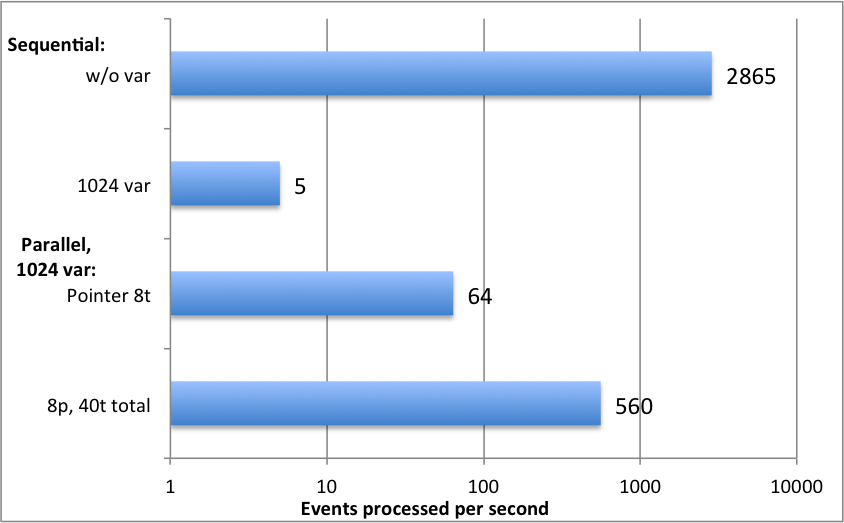
\includegraphics[scale=0.55]{charts/events_per_sec.png}
		\caption{Throughput of events processed for the original sequential \tth,with no and 1024 variations (\textit{var}), and for the parallel pointer and multiprocess implementations (with \textit{t} being threads and \textit{p} processes).}
		\label{fig:events_sec}
	\end{center}
\end{figure}

Figure \ref{fig:events_sec} plots the number of events processed per second in the original sequential application without variations of the particle characteristics, for 1024 variations, and for the parallel pointer and multiprocess implementations for 1024 variations. Using a single process, the throughput improves by a factor of 12.8, from 5 to 64 events per second, using a single CPU device. The best overall performance, for the multiprocess implementation with 8 processes with 5 threads each, provided an improvement by a factor of 113 on event throughput, from 5 to 560 events per second. Note that these results were obtained on a single computer with a dual 10-core Xeon, without using accelerators yet.

Other issues may also affect the code execution efficiency, but they were considered out of the scope of this communication. The compiler, and respective optimization options, can have a big impact in application performance, where different options may be best suited for certain applications than others. Rules for writing vectorized code were not presented but may improve the efficiency when processing large amounts of data, as the compiler is not able to perform most code modifications necessary to take advantage of vector instructions. Using efficient numeric libraries \cite{MKL,BLAS} when required usually has a big impact on performance. There are guides that provide rules and present techniques for developing efficient code \cite{Intel:Optimization,Intel:DevOptimization,NUMA}.

These promising results on code execution efficiency leave yet some room for further enhancements. The scheduler could be improved to automatically predict the best process/thread configuration for each system by analysing a set of micro-benchmarks or the application itself on a small input, and ultimately identify the best core affinity scheme. Also, the application efficiency could be improved using hardware accelerators, balancing the workload among accelerators and CPU devices in heterogeneous systems. The use of development frameworks for heterogeneous systems, such as StarPU \cite{StarPU}, may further improve productivity and efficiency through aids in code parallelization and transparent workload distribution among multi-core devices and computing accelerators.
